\section{Item b)}

Considerando a permeabilidade magnética do núcleo infinita, a relutânciaConsiderando a permeabilidade magnética do núcleo infinita, a relutância do ferro é nula e a relação entre a FMM espacial e a densidade de fluxo no entreferro torna-se direta:
\[
B_g(\theta)=\frac{\mu_0}{g}\,F(\theta).
\]

A FMM produzida por um enrolamento distribuído pode ser decomposta em série de Fourier. Para a harmônica espacial de ordem \(v\), a amplitude da componente de \(B_g\) é proporcional ao fator de enrolamento harmônico \(k_{w,v}\) e inversamente proporcional a \(v\)~\cite{FitzgeraldKingsleyUmans2014,Chapman2013MaquinasEletricas}. Normalizando pela componente fundamental, obtém-se
\[
\frac{|B_v|}{|B_1|}=
\frac{|k_{w,v}|}{v\,|k_{w,1}|}
\quad\Rightarrow\quad
|B_v|
=
0{,}9\,
\frac{|k_{w,v}|}{v\,|k_{w,1}|}
\quad[\mathrm{T}],
\]

Para as configurações de passo pleno, tem-se \(\rho=180^\circ\) e, em módulo,
\[
|k_{p,v}|=\left|\sin(v\cdot90^\circ)\right|=1
\]
para todo \(v\) ímpar. Portanto, no modelo analítico ideal, as configurações de camada simples e camada dupla com passo pleno apresentam espectros numericamente idênticos, pois possuem a mesma distribuição espacial efetiva dos lados de bobina~\cite{FitzgeraldKingsleyUmans2014}. Para a configuração de camada dupla e passo encurtado de \(5/6\), tem-se \(\rho=150^\circ\). Logo,
\[
|k_{p,5}|
=
\left|\sin\left(\frac{5\cdot150^\circ}{2}\right)\right|
=
0{,}2588,
\quad
|k_{p,7}|
=
\left|\sin\left(\frac{7\cdot150^\circ}{2}\right)\right|
=
0{,}2588.
\]

Combinando esses valores com \(|k_{d,5}|=|k_{d,7}|=0{,}2588\), obtém-se \(|k_{w,5}|=|k_{w,7}|=0{,}0670\).
Assim, as amplitudes de \(B_5\) e \(B_7\) passam de \(0{,}0482\,\mathrm{T}\) e \(0{,}0345\,\mathrm{T}\), no caso de passo pleno, para \(0{,}0129\,\mathrm{T}\) e \(0{,}0092\,\mathrm{T}\), respectivamente, no caso de passo encurtado. Isso representa uma atenuação de aproximadamente \(73\%\) nessas componentes~\cite{Chapman2013MaquinasEletricas}.

Portanto, configurações de camada simples e camada dupla com passo pleno (C1 e C2), nenhuma harmônica ímpar é eliminada pelo enrolamento, as harmônicas de \(5^\mathrm{a}\) e \(7^\mathrm{a}\) ordens estão presentes com amplitudes de \(0{,}0482\,\mathrm{T}\) e \(0{,}0345\,\mathrm{T}\), respectivamente, sendo as triplas canceladas pelo sistema trifásico. Para a configuração de camada dupla com passo encurtado de \(5/6\) (C3), as harmônicas de \(5^\mathrm{a}\) e \(7^\mathrm{a}\) ordens são fortemente atenuadas, enquanto as de \(11^\mathrm{a}\) e \(13^\mathrm{a}\) ordens permanecem praticamente inalteradas.
A tabela a seguir resume os resultados obtidos para as componentes de \(B_g\) de ordem \(v=1,3,5,7,9,11,13\) para as três configurações de enrolamento analisadas.
\[
\begin{array}{c c c c c}
    \hline
    v &
    |B_{v,\mathrm{fase}}|\;\text{C1/C2 [T]} & \text{Situação no 3}\phi &
    |B_{v,\mathrm{fase}}|\;\text{C3 [T]} & \text{Situação no 3}\phi \\
    \hline
    1  & 0{,}9000 & Presente            & 0{,}9000 & Presente \\
    3  & 0{,}2196 & Suprimida (3\phi)   & 0{,}1608 & Suprimida (3\phi) \\
    5  & 0{,}0482 & Presente            & 0{,}0129 & Atenuada (-73\%) \\
    7  & 0{,}0345 & Presente            & 0{,}0092 & Atenuada (-73\%) \\
    9  & 0{,}0732 & Suprimida (3\phi)   & 0{,}0536 & Suprimida (3\phi) \\
    11 & 0{,}0818 & Presente            & 0{,}0818 & Presente \\
    13 & 0{,}0692 & Presente            & 0{,}0692 & Presente \\
    \hline
\end{array}
\]

% \begin{figure}[htbp]
%     \centering
%     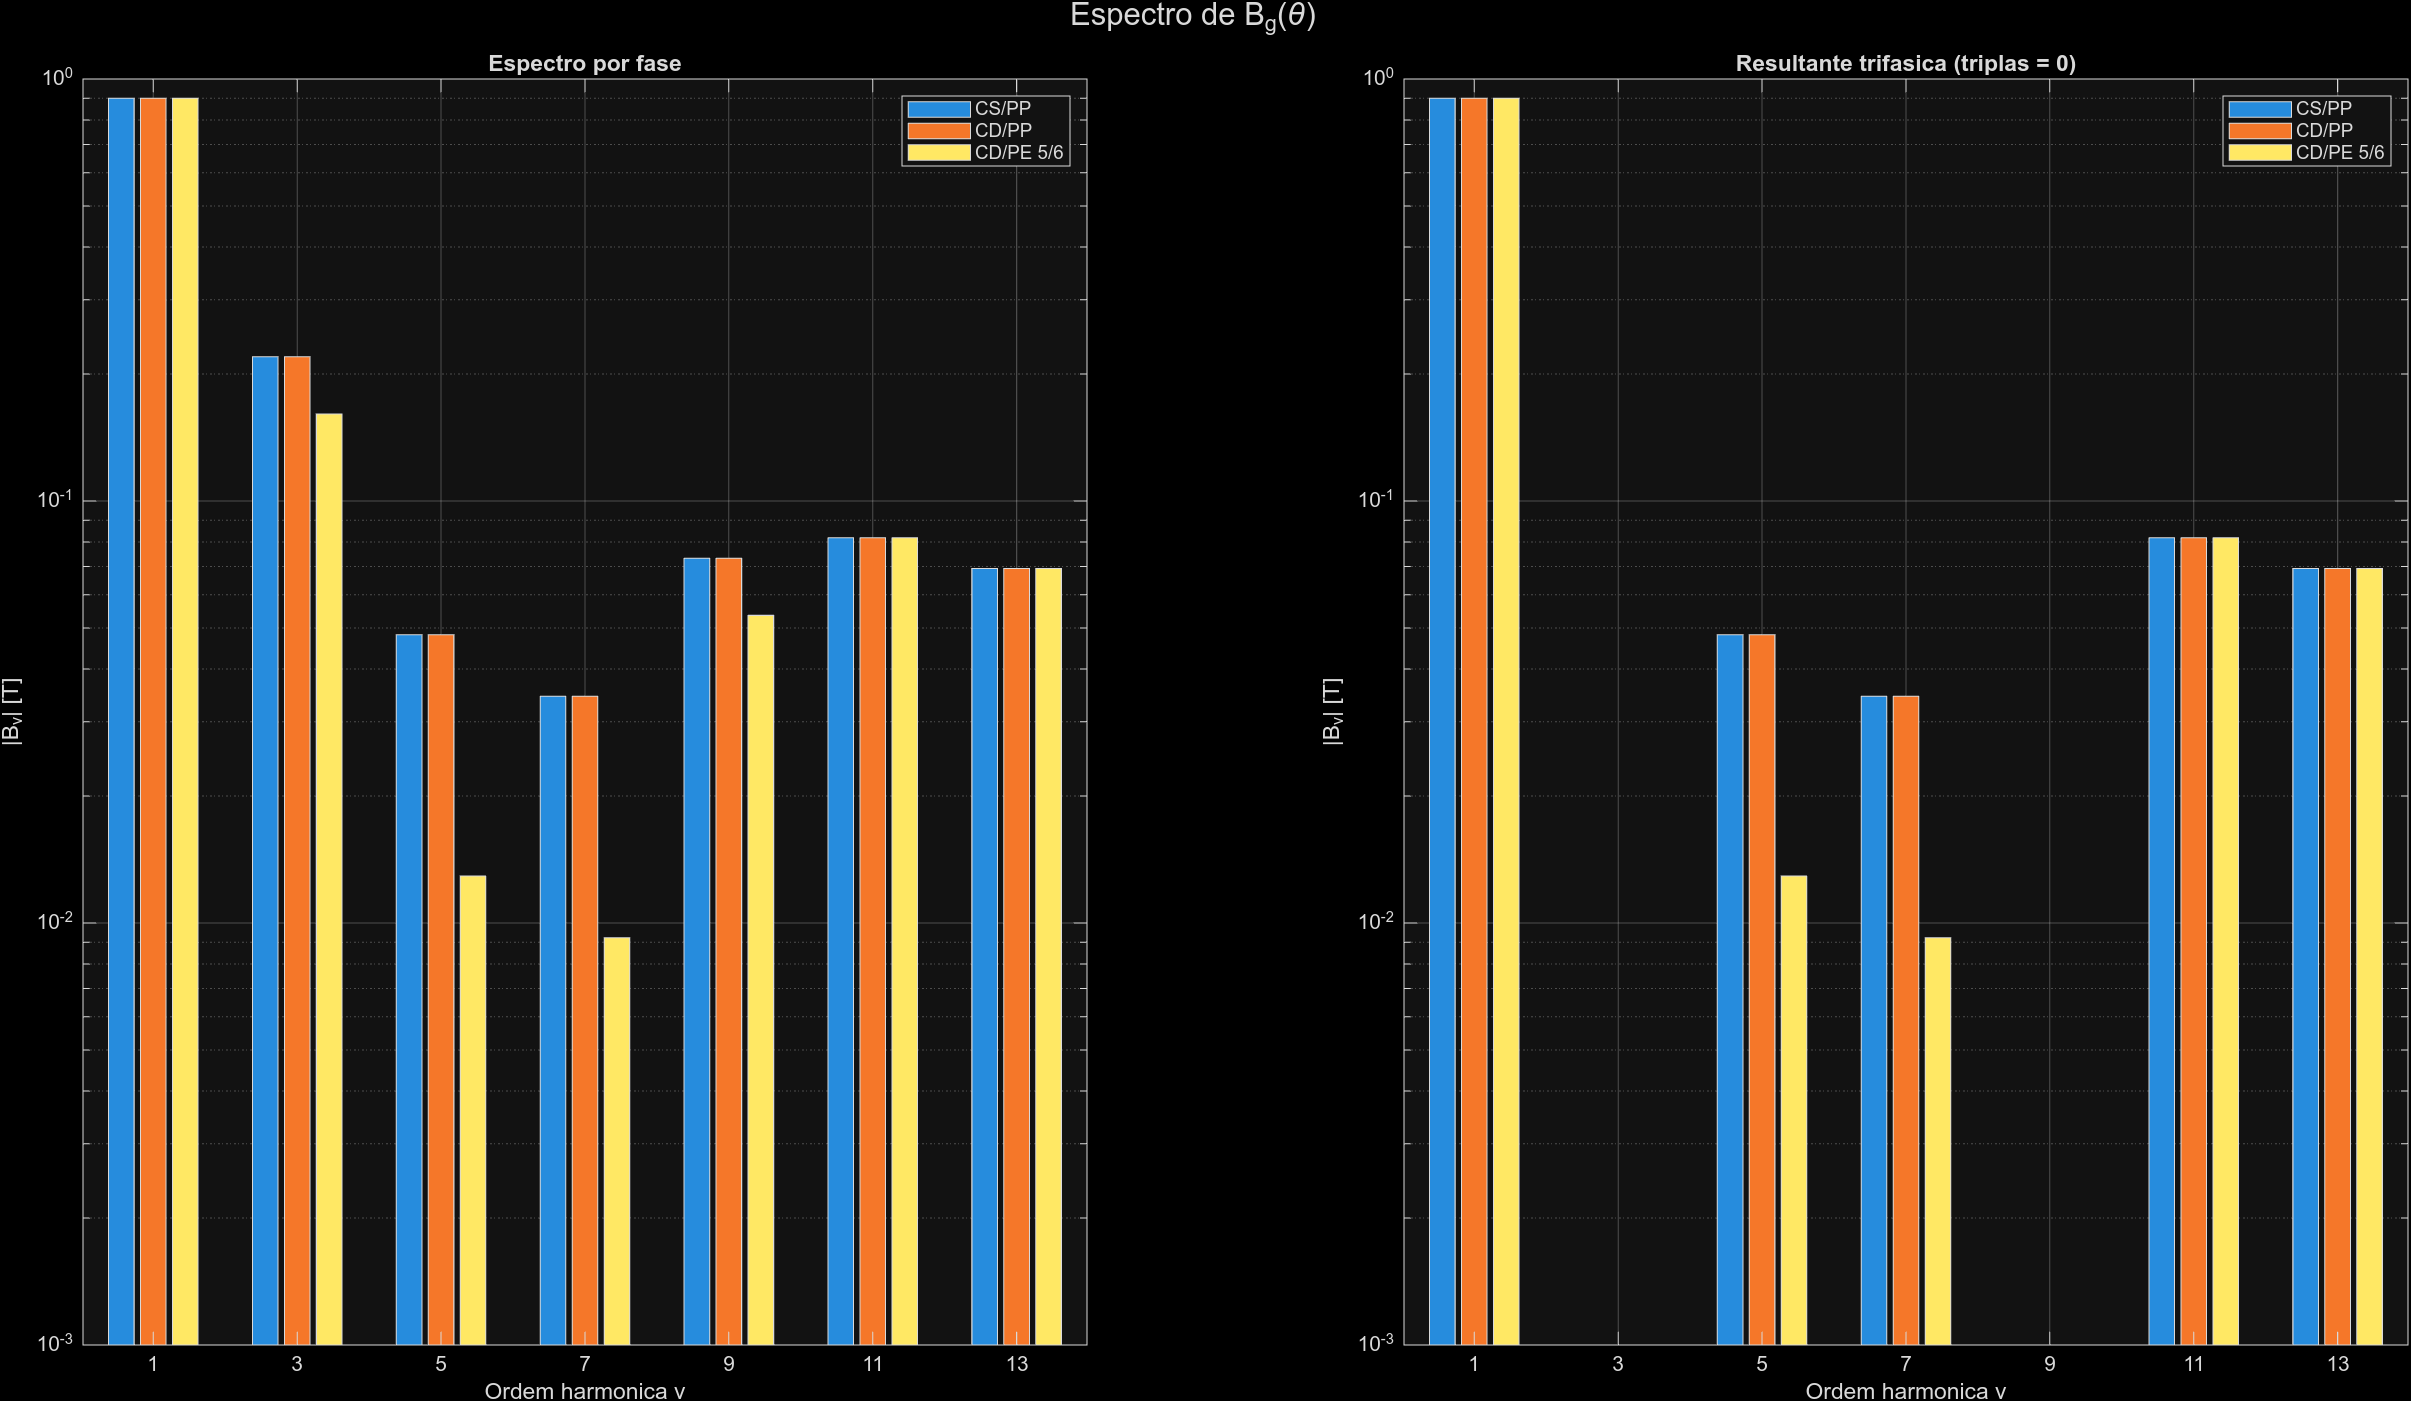
\includegraphics[width=0.55\linewidth]{../img/espctro_de_b.png}
%     \caption{Espectro harmônico de \(B_g(\theta)\) para as três configurações de enrolamento.}
%     \label{fig:espectro_bg}
% \end{figure}
